\documentclass[hidelinks,10pt,a4paper]{article}
\usepackage[T1]{fontenc}
\usepackage[polish]{babel}
\usepackage[utf8]{inputenc}
\usepackage{lmodern}
\selectlanguage{polish}
\usepackage{amsmath}
\usepackage{amsfonts}
\usepackage{pdfpages}
\usepackage{hyperref}
\newcommand\tab[1][0.5cm]{\hspace*{#1}}


\begin{document}
\title{Algorytmy i Struktury Danych \\ projekt grupowy \\ specyfikacja funkcjonalna programu \\``Program''}
\author{Bazyli Reps}
\maketitle

\newpage

\tableofcontents

\newpage

\section{Wstęp}
\tab Celem projektu jest napisanie aplikacji umożliwiającej dzielenie obszaru na obszary na podstawie dostarczonych przez użytkownika współrzędnych miejsc symbolizujących instytucje finansowe, nazywane w dalszej części dokumentu \textbf{punktami kluczowymi}.
Aplikacja ta w dalszej części dokumentu będzie nazywana programem.

Poza punktami kluczowymi użytkownik dostarcza także informację dotyczącą \textbf{konturów}, czyli zbioru \textbf{współrzędnych} wyznaczających granicę symulowanego obszaru oraz \textbf{obiektów}, czyli określonych przez użytkownika bytów posiadających określone właściwości i znajdujących się na danym obszarze. Dane dostarczane są z pliku tekstowego zwanego dalej \textbf{plikiem wejściowym} lub z programu.
Dokładne informacje dotyczące podmiotów wypisanych pogrubioną czcionką znajdują się w sekcji \hyperref[sec:daneWej]{\textit{4 Format danych}}.

\section{Wymagania funkcjonalne}
\tab Program ma zawierać nastepujące funkcjonalności:
\begin{enumerate}


\item rysowanie i wczytywanie danych takich bytów jak:
\begin{enumerate}
\item \textbf{punkty kluczowe}
\item \textbf{kontury}
\item \textbf{obiekty}
\end{enumerate}
przy czym \textbf{punkty kluczowe} oraz \textbf{kontury} mają ściśle zdefiniowaną w tym dokumencie listę atrybutów, natomiast \textbf{obiekty} mają atrybuty definiowane przez użytkownika,
\item wyznaczanie i rysowanie granic na podstawie \textbf{konturów},
\item wyznaczenie i narysowanie optymalnych granic obszarów dookoła \textbf{punktów kluczowych}, nazywanych dalej \textbf{obszarami} przy czym:
\begin{enumerate}
\item w każdym z takich \textbf{obszarów} znajduje się wyłącznie jeden punkt kluczowy
\item optymalne granice mają wyznaczać takie \textbf{obszary}, w których każdy punkt należący do \textbf{obszaru} znajduje się bliżej \textbf{punktu kluczowego} tego \textbf{obszaru} niż jakiegokolwiek innego \textbf{punktu kluczowego}
\end{enumerate}
\item wyświetlanie posegregowanej według typów listy \textbf{obiektów} należących do każdego \textbf{obszaru}
\item tworzenie oraz wyświetlanie na żądanie użytkownika statystyk dotyczących danego obszaru, gdzie przez statystyki rozumie się:
\begin{enumerate}
\item podawanie liczby mieszkańców na podstawie informacji o \textbf{obiektach} zawierających atrybut typu \textit{L\_MIESZKANCOW} znajdujących się na \textbf{obszarze} 
\item wyznaczenie typów \textbf{obiektów} znajdujących się na \textbf{obszarze} oraz podanie ilości instancji \textbf{obiektów} dla każdego z typów
\end{enumerate}
\item podczas działania programu dodawanie i usuwanie elementów \textbf{konturów}
\item podczas działania programu dodawanie i usuwanie \textbf{punktów kluczowych} 
\item podkładanie pod rysowane \textbf{kontury} grafiki dostarczonej przez użytkownika

\end{enumerate}



\section{Wymagania niefunkcjonalne}
\tab Program ma pracować jako aplikacja internetowa, co oznacza, że będzie działał on na serwerze dostawcy usług a klient będzie komunikował się z nim przez przeglądarkę internetową za pomocą sieci WWW.
\subsection{obsługiwane przeglądarki}
Program ma być obsługiwany przez aktualne w czasie utworzenia dokumentu  przeglądarki internetowe takie jak:
\begin{itemize}
\item Mozilla Firefox
\item Google Chrome
\item Safari
\item Microsoft Edge
\end{itemize}  
\subsection{wykorzystywane technologie}
Program ma być napisany z wykorzystaniem następujących technologii [lista technologii]




\section{Format danych}
\label{sec:daneWej}

\subsection{pliki}
Użytkownik opcjonalnie dostarcza programowi następujące pliki:
\begin{enumerate}
\item Tekstowy plik o rozszerzeniu \textit{.txt} z enkodowaniem \textit{utf-8} zawierający informacje dotyczące \textbf{konturów}, \textbf{punktów kluczowych} oraz \textbf{obiektów} nazywany \textbf{plikiem wejściowym}
\item Grafikę w jednym z następujących formatów: 
\begin{enumerate}
\item .png
\item .jpg
\item .jpeg
\item .bmp
\item .gif
\end{enumerate}
która może służyć jako tło dla rysowanego układu nazywaną dalej   \textbf{grafiką}.
\end{enumerate}

\subsection{przykład poprawnie sformatowanego pliku wejściowego}
\# Kontury terenu (wymienione w kolejności łączenia): Lp. x y
\\1. 0 0
\\2. 0 20
\\3. 20 30
\\4. 40 20
\\5. 40 0
\\
\\
\# Punkty kluczowe: Lp. x y Nazwa
\\1. 1 1 KOK Krawczyka
\\2. 1 19 KOK Kaczmarskiego
\\3. 30 10 KOK Łazarewicza
\\
\\
\# Definicje obiektów: Lp. Typ\_obiektu (Nazwa\_zmiennej Typ\_zmiennej)
\\1. SZKOŁA Nazwa string X double Y double
\\2. DOM X double Y double L\_MIESZKAŃCÓW int
\\3. NIEDŹWIEDŹ X double Y double
\\
\\
\# Obiekty: Typ\_obiektu (zgodnie z definicją)
\\1. SZKOŁA "Szkoła robienia dużych pieniędzy" 4 1
\\2. DOM 4 3 100
\\3. DOM 4 17 120
\\4. DOM 4 18 80
\\5. NIEDŹWIEDŹ 20 20
\\6. NIEDŹWIEDŹ 40 1
\\7. NIEDŹWIEDŹ 39 1
\\8. NIEDŹWIEDŹ 39 2
\\
\subsection{opis typów}


\subsubsection{kontury / współrzędna}
\textbf{Kontury} stanowią listę obiektów typu \textbf{współrzędna}.
Kolejność w liście odwzorowuje kolejność dodawania \textbf{współrzędnych} do listy w ten sposób, że pierwsza dodana do \textbf{konturów} \textbf{współrzędna} będzie pierwszą \textbf{współrzędną} na liście. Każda z \textbf{współrzędnych} zawiera dokładnie dwa atrybuty:
\begin{enumerate}
\item \textit{x} - nieujemna liczba całkowita oznaczająca wartość odciętych w dwuwymiarowym układzie współrzędnych
\item \textit{y} - nieujemna liczba całkowita oznaczająca wartość rzędnych w dwuwymiarowym układzie współrzędnych
\end{enumerate}

\subsubsection{punkt kluczowy}
\textbf{Punkt kluczowy} symbolizuje instytucję finansową. 
Zawiera on dokładnie trzy atrybuty:
\begin{enumerate}
\item \textit{x} - nieujemna liczba całkowita oznaczająca wartość odciętych w dwuwymiarowym układzie współrzędnych
\item \textit{y} - nieujemna liczba całkowita oznaczająca wartość rzędnych w dwuwymiarowym układzie współrzędnych
\item \textit{Nazwa} - nazwa instytucji. Całość nazwy razem ze spacjami lub innymi białymi znakami nie może przekraczać 100 znaków. 
\end{enumerate}

\subsubsection{obiekt}
\textbf{Obiekt} jest definiowany przez użytkownika w \textbf{pliku wejściowym} lub bezpośrednio w programie. 
\textbf{Obiekt} może zawierać od dwóch do sześciu atrybutów pośród których koniecznie muszą znaleźć się dwa atrybuty:
\begin{enumerate}
\item \textit{x} - nieujemna liczba całkowita oznaczająca wartość odciętych w dwuwymiarowym układzie współrzędnych
\item \textit{y} - nieujemna liczba całkowita oznaczająca wartość rzędnych w dwuwymiarowym układzie współrzędnych
\end{enumerate}
Atrybuty w \textbf{obiekcie} mogą być dodawane w dowolnej kolejności.

\subsection{opis formatowania}
\begin{enumerate}


\item \textbf{Plik wejściowy} musi składać się z dokładnie czterech sekcji, z których każda z nich musi zaczynać się linią w której pierwszym znakiem jest znak '\#' zwaną dalej \textbf{linią rozpoczynającą}.
\item W dalszej części \textbf{linii rozpoczynającej} użytkownik może wpisać dowolne znaki. 
\item Linie następujace po \textbf{linii rozpoczynającej} w każdej sekcji nazywane są \textbf{liniami deklaracji}.
\item Każda \textbf{linia deklaracji} ma zawierać deklarację pojedynczego bytu i każdy byt musi być zadeklarowany w dokładnie jednej \textbf{linii deklaracji}.
\item Każda z linii nie może zawierać więcej niż 200 znaków.
\item \textbf{Linie deklaracji} w każdej sekcji muszą być numerowane kolejnymi liczbami naturalnymi (rozpoczynając od liczby '1') po których bezpośrednio występuje znak kropki '.' i co najmniej jedna spacja, przy czym w każdej sekcji numerowanie następuje od '1'. Figura taka (liczba-kropka-spacja) nazywana jest \textbf{numerem linii}.
\item Kolejne wyrazy w \textbf{linii deklaracji} muszą być oddzielone co najmniej jedną spacją. Wyrazy nie będące \textbf{numerem linii} są nazywane \textbf{elementami}.
\end{enumerate}
 

\subsubsection{kontury}
Sekcja ta może zawierać co najwyżej 1000 \textbf{linii deklaracji}.
Każda \textbf{linia deklaracji} tej sekcji musi zawierać dokładnie dwa \textbf{elementy} oznaczające atrybuty \textit{X} i \textit{Y} opisane w podpunkcie 4.3.1.
\\ Kolejność: [\textbf{numer linii}] [X] [Y]

\subsubsection{punkty kluczowe}
Sekcja ta może zawierać co najwyżej 10000 \textbf{linii deklaracji}.
Każda \textbf{linia deklaracji} tej sekcji musi zawierać dokładnie trzy \textbf{elementy} oznaczające atrybuty \textit{X}, \textit{Y}, \textit{Nazwa} opisane w podpunkcie 4.3.2. W tej sekcji \textbf{element} \textit{Nazwa} może składać się z wielu wyrazów. Tworzony jest on przez wszystkie wyrazy napotkane w \textbf{linii deklaracji} po napotkaniu w niej \textbf{elementów} \textit{X} i \textit{Y}.
\\
\\ Kolejność: [\textbf{numer linii}] [X] [Y] [Nazwa$_{1}$] ... [Nazwa$_{n}$]

\subsubsection{definicje obiektów}
Sekcja ta może zawierać co najwyżej 1000 \textbf{linii deklaracji}.
Każda \textbf{linia deklaracji} musi zawierać co najmniej 5 \textbf{elementów}. 
Pierwszy \textbf{element} musi być napisem oznaczającym typ \textbf{obiektu} i musi być pierwszym \textbf{elementem} w \textbf{linii deklaracji}.
Pozostałe cztery wymagane \textbf{elementy} są to dwie pary \textbf{elementów} (X, double) i (Y, double) oznaczających atrybuty \textit{X} i \textit{Y} \textbf{obiektów} opisane w podpunkcie 4.3.3. Pary mogą znaleźć się na dowolnej pozycji w \textbf{linii deklaracji} poza pozycją pierwszą. \textbf{Elementy} w parze są nierozłączne.
Łącznie w jednej \textbf{linii deklaracji} może znajdować się sześć par (nazwa atrybutu, typ atrybutu).
Typy muszą być pisane małymi literami.
\\\\Kolejność: [\textbf{numer linii}] [Atrybut$_{1}$] [Typ atrybutu$_{1}$] ... [Atrybut$_{n}$] [Typ atrybutu$_{n}$]
\section{Obsługa programu}

\subsection{Schemat interfejsu}
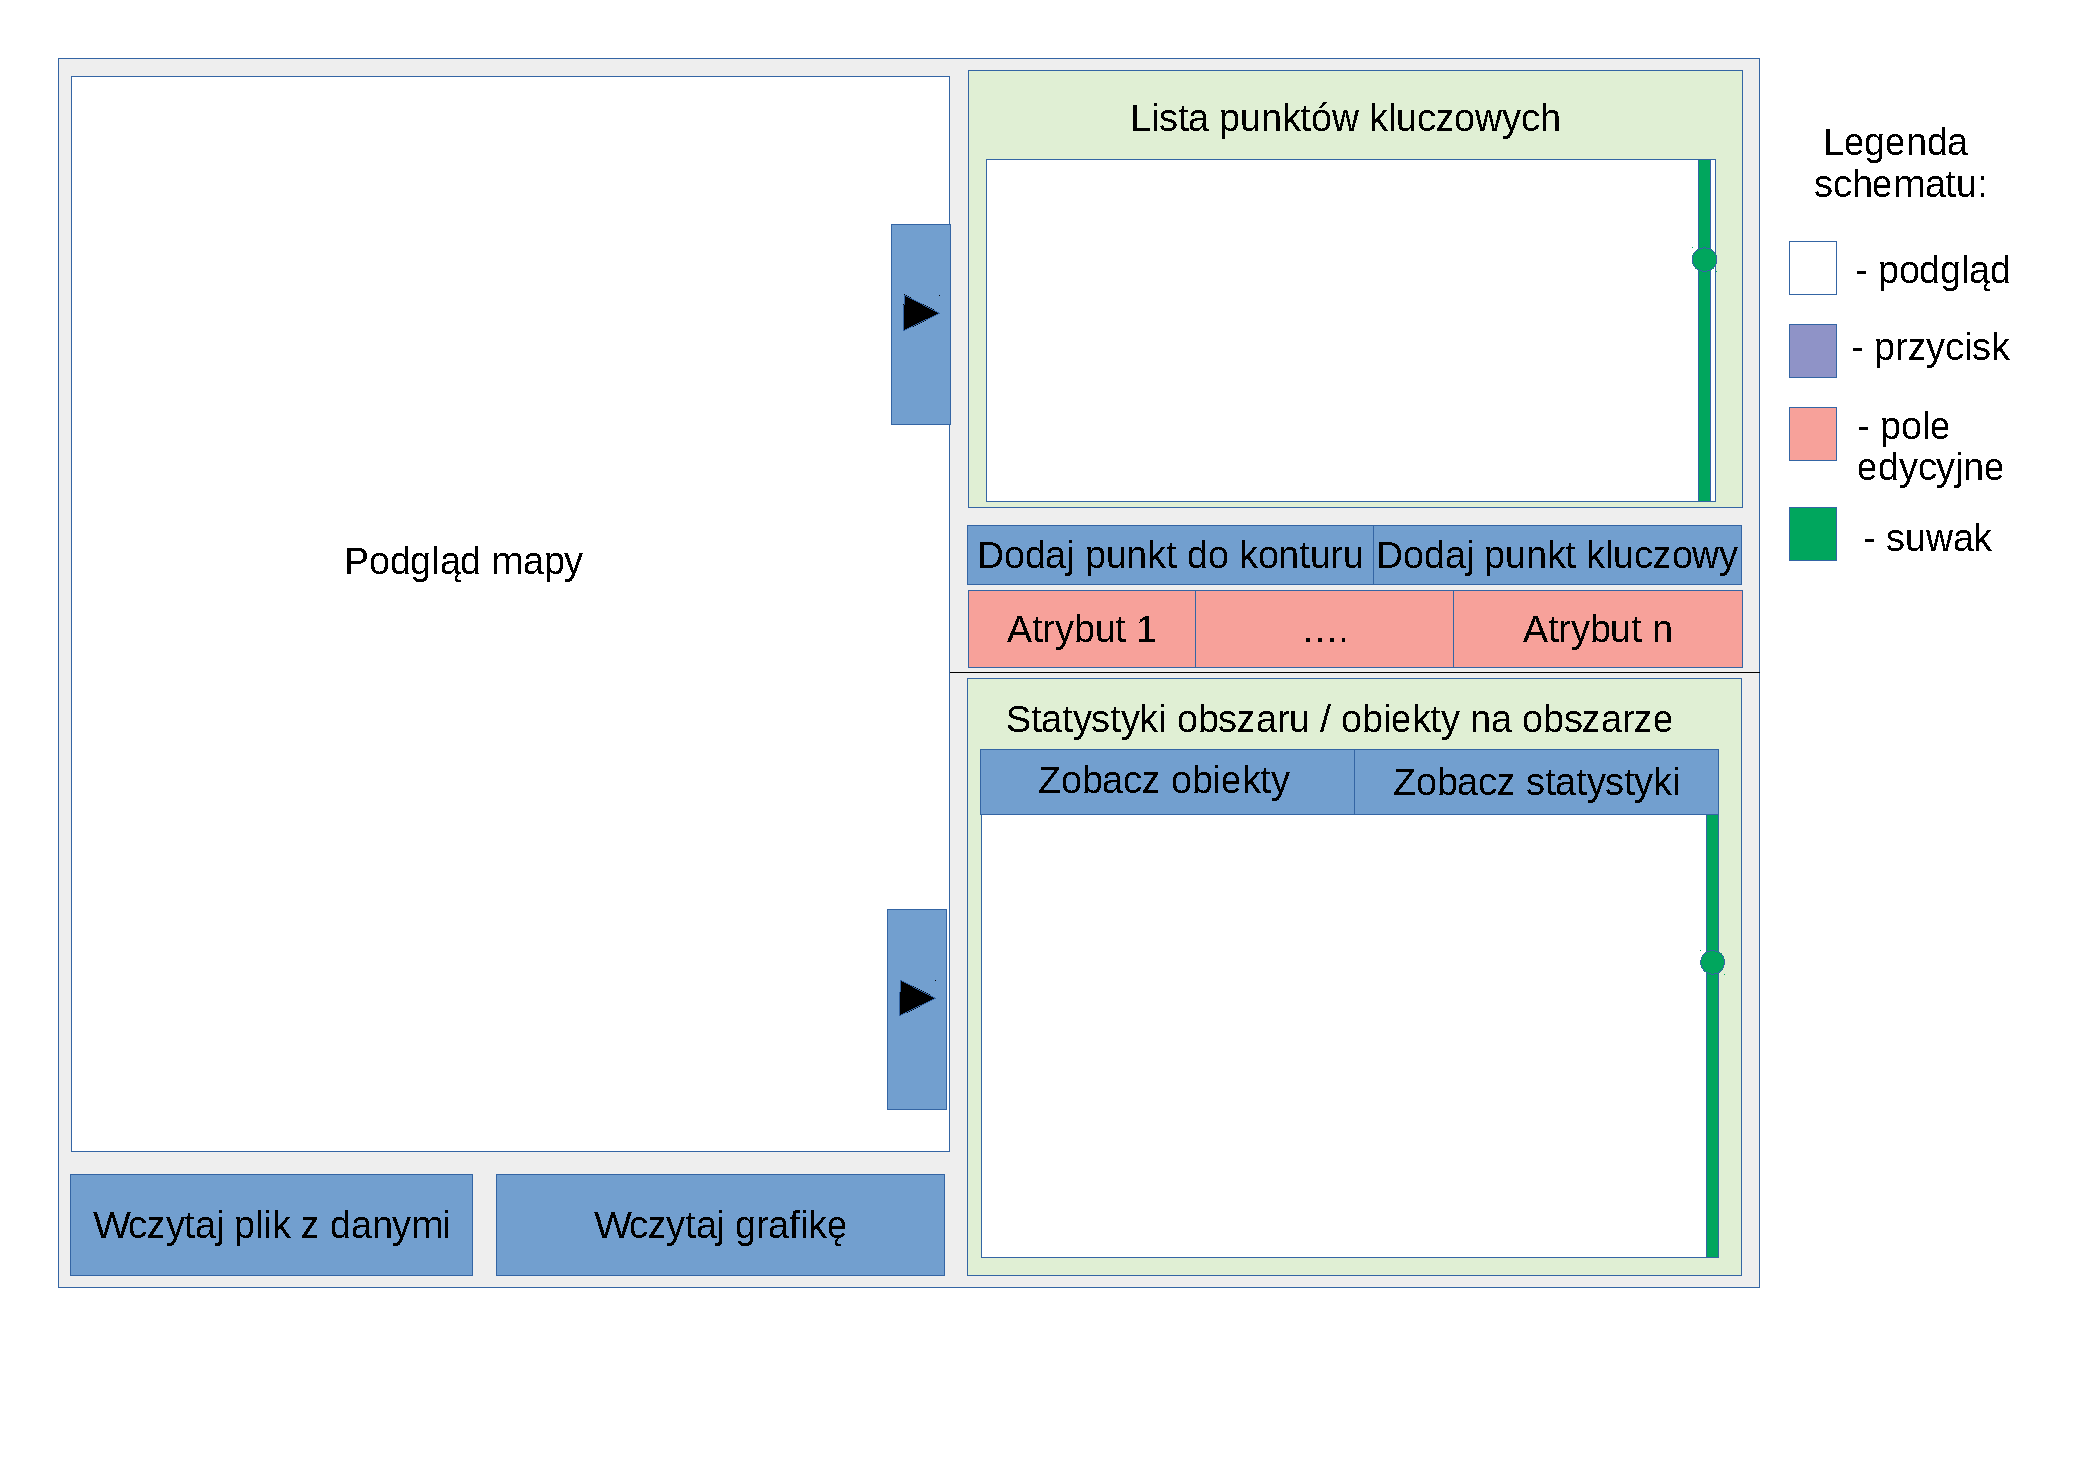
\includegraphics[width = \textwidth]{gui.pdf}

\subsection{Opis działania programu}
\subsubsection{uruchomienie programu}
Użytkownik uruchamia program poprzez uruchomienie przeglądarki internetowej i wejście na adres [adres aplikacji]. 
\subsubsection{wczytywanie pliku wejściowego lub grafiki}
Użytkownik wczytuje plik wejściowy lub grafikę poprzez kliknięcie przycisku \textbf{Wczytaj plik z danymi} lub \textbf{Wczytaj grafikę} i wybranie w wyświetlonym okienku wyboru pliku pożądanego pliku.
\subsubsection{przeglądanie mapy}
Użytkownik przegląda mapę, jeżeli nie mieści się ona w całości w okienku, poprzez używanie strzałek na klawiaturze. 
\subsubsection{wyświetlanie statystyk lub listy obiektów należących do danego obszaru}
Użytkownik wyświetla statystyki danego obszaru poprzez kliknięcie myszą na mapie na interesującym go obszarze i kliknięcie przycisku \textbf{Zobacz statystyki} lub przycisku \textbf{Zobacz obiekty}.
\subsubsection{dodawanie punktu do konturu}
Użytkownik dodaje punkt do konturów poprzez kliknięcie przycisku \textbf{Dodaj punkt do konturu}.
Po wykonaniu tej akcji uaktywnią się dwa pola edycyjne poniżej przycisku.
W pierwszym z nich należy podać współrzędną \textit{X}, a w drugim współrzędną \textit{Y} a następnie jeszcze raz nacisnąć przycisk \textbf{Dodaj punkt do konturu}.
\subsubsection{dodawanie punktu kluczowego}
Użytkownik dodaje punkt kluczowy poprzez kliknięcie przycisku \textbf{Dodaj punkt kluczowy}.
Po wykonaniu tej akcji uaktywnią się pola edycyjne poniżej przycisku.
W pierwszym z nich należy podać współrzędną \textit{X}, w drugim współrzędną \textit{Y}, w trzecim podać nazwę punktu kluczowego a następnie jeszcze raz nacisnąć przycisk \textbf{Dodaj punkt kluczowy}.
\subsubsection{chowanie listy punktów kluczowych lub statystyk}
Użytkownik może schować listę punktów kluczowych lub statystyki poprzez kliknięcie przycisku z czarnym trójkątem znajdującego się na wysokości wybranego elementu.
Aby przywrócić ich widok należy jeszcze raz nacisnąć na dany przycisk.




\section{Sytuacje wyjątkowe}
\tab W przypadku wystąpienia sytuacji wyjątkowej program wypisze w przeglądarce odpowiedni komunikat oraz w razie konieczności zaznaczy miejsce w którym popełniono błąd kolorem czerwonym.

\subsection{Błędy pliku}
\begin{enumerate}


\item{\textbf{Nie można otworzyć wybranego pliku}}
\\komunikat: Nie mogę otworzyć wybranego pliku [nazwa pliku]!  
\item \textbf{Nieodpowiedni format pliku}
\begin{enumerate}
\item \textbf{plik wejściowy}
\\ komunikat: Plik wejściowy jest w nieodpowiednim formacie! Plik wejściowy musi być plikiem tekstowym z enkodowaniem UTF-8! 
\item \textbf{grafika}
\\ komunikat: Grafika jest w nieodpowiednim formacie! Grafika powinna być w jednym z formatów: JPG, JPEG, PNG, GIF, BMP! 
\end{enumerate}
\end{enumerate}

\subsection{Błędy formatowania pliku}
\tab W przypadku wystąpienia jakiejkolwiek sytuacji wyjątkowej na wszelki wypadek \textbf{plik wejściowy} nie zostanie wczytany.
\begin{enumerate} 

\item \textbf{Błędny typ danych w danym miejscu:}
\\
\\komunikat: W pliku [\textit{nazwaPliku}] w linii [\textit{nrLinii}] znaleziono ciąg znaków [\textit{ciągZnaków}]. W tym miejscu powinna się znajdować [\textit{pożądana wartość, np. liczba całkowita określająca wartość atrybutu X}]!

\item \textbf{Nieodpowiedni format liczby oznaczającej współrzędne lub liczbę mieszkańców}
\\\\komunikat: W pliku [nazwa pliku] w linii [numer linii] znaleziono liczbę [znaleziona liczba]. W tym miejscu musi znajdować się nieujemna liczba całkowita!

\item \textbf{Nierozpoznany typ zmiennej}
\\\\komunikat: W pliku [nazwa pliku] w linii [numer linii] w sekcji DEFINICJA OBIEKTÓW natrafiono na nierozpoznany tym zmiennej [dana zmienna]. Dopuszczalne typy zmiennych to: string, int, double.

\item \textbf{Błędne numerowanie linii deklaracji}
\\\\komunikat: W pliku [nazwa pliku] w linii [numer linii] znaleziono nieodpowiednio numerowaną linię deklaracji! Linie deklaracji muszą być kolejnymi liczbami naturalnymi. Linie deklaracji każdej sekcji muszą rozpoczynać się od jedynki.

\item \textbf{Więcej elementów w linii niż jest dozwolone.}
\\
\\komunikat: W pliku [\textit{nazwa pliku}] w linii [\textit{nrLinii}] znajduje się [\textit{liczba elementów}]. Dozwolona liczba elementów w danej linii to [\textit{liczba elementów}].

\item \textbf{Więcej znaków w linii niż dozwolone}
\\\\komunikat: W linii [numer linii] znajduje się [liczba znaków]. Maksymalna dopuszczalna liczba znaków w linii wynosi [maksymalna ilość znaków]!

\item \textbf{Więcej linii w sekcji niż jest dozwolone}
\\\\komunikat: W pliku [nazwa pliku] w sekcji [typ sekcji, np. kontury] znaleziono [liczba linii] linii. Maksymalna liczba linii w tej sekcji wynosi [maksymalna liczba linii].

\item \textbf{Brak dostatecznej ilości informacji w linii}
\\\\komunikat: W pliku [nazwa pliku] w linii [numer linii] znaleziono za mało elementów. Odpowiednia liczba elementów to [odpowiednia liczba]. Znaleziono: [ilosć znalezionych].

\item \textbf{Powtórzona deklaracja obiektu.}
\\
\\komunikat: W pliku [\textit{nazwa pliku}] w linii [\textit{nrLinii}] natrafiono na ponowną deklarację obiektu typu[\textit{typ obiektu i linia pierwszej deklaracji}].

\item \textbf{Dwa byty znajdują się na tych samych współrzędnych}
\\
\\komunikat: W pliku [nazwa pliku] naleziono dwa byty o tych samych współrzędnych pod liniami [numer linii1] i [numer linii2]! Każdy byt musi znajdować się na niepowtarzalnych współrzędnych!

\item \textbf{Nieodpowiednia ilość linii rozpoczynających}
\\\\komunikat: Znaleziono [liczba linii] linii rozpoczynających (zaczynających się od \#). Każda sekcja musi zaczynać się od linii rozpoczynającej, więc muszą wystąpić co najmniej 4 takie linie!

\end{enumerate}

\subsection{Błędy występujące po wczytaniu pliku}

\begin{enumerate}

\item \textbf{Punkt kluczowy lub obiekt znajduje się poza konturami}
\\\\komunikat: [Typ bytu] znajduje się poza podanymi konturami. Wszystkie punkty kluczowe oraz obiekty muszą znajdować się wewnątrz obszaru wyznaczonego przez kontury.

\item \textbf{Podane nieprawidłowe dane podczas dodawania nowego punktu kluczowego bądź elementu konturów}
\\\\komunikat: [Typ atrybutu] musi być [opis poprawnie podanego atrybutu]!

\item \textbf{Próba dodania punktu kluczowego, konturu lub obiektu powyżej limitu ilości}
\\\\komunikat: Nie dodano nowego [rodzaj bytu]! Maksymalna ilość [rodzaj bytu] wynosi [maksymalna ilość dla danego rodzaju]!

\end{enumerate}

\section{Testy akceptacyjne}





\end{document}
